\chapter{Background and State of the Art}\makeatletter\def\@currentlabel{3}\makeatother
\label{chap1}
\lhead{\textbf{CHAPTER 1.} \textit{Background and State of the Art}}
This chapter offers a compact map of the knowledge needed to follow the rest of the thesis. We start with the building blocks of public blockchains: hash functions, Merkle trees, digital signatures, and the two dominant consensus schemes, Proof-of-Work and Proof-of-Stake. Then, zoom in on Bitcoin’s UTXO ledger and Ethereum’s smart-contract account model, the specific terrain on which our exploits run. Next, we sketch the evolution of zero-knowledge proofs, from early interactive protocols to today’s fast SNARK/STARK systems, before introducing zero-knowledge virtual machines (zkVMs), the technology that lets us prove an entire program’s execution without revealing its data. These three threads provide the conceptual toolkit that the subsequent chapters will apply when presenting and evaluating \textit{zkpoex}. 

\section{Brief Introduction to Blockchain}\label{sec:blockchain_intro}

A blockchain can be understood as a publicly distributed digital ledger that maintains transactions among members of a network. These transactions are assembled into sequential blocks, each referencing the previous one according to specific rules and data structures. A pivotal aspect of blockchain technology is that after a block is appended to the chain, any subsequent alteration demands the modification of all blocks that follow it, making tampering highly impractical.

The conceptual origins of this technology can be traced to David Chaum's 1982 doctoral research at the University of California, titled \textit{“Computer Systems Established, Maintained and Trusted by Mutually Suspicious Groups”} \cite{Cha82}. Subsequent exploration into a cryptographically protected chain of blocks was documented in 1991 by Stuart Haber and W. Scott Stornetta \cite{HaberStornetta1991}, who aimed to establish a tamper-resistant mechanism for document timestamps. The following year, in collaboration with Dave Bayer, they enhanced the design by integrating Merkle trees, an improvement that allowed multiple document certificates to be batched into a single block, thereby increasing efficiency \cite{HaberStornettaBayer1992}.

Later, Wei Dai's b-money proposal \cite{DaiBmoney} introduced, in 1998, the idea of creating currency by solving computational challenges and contemplated achieving consensus through interactions among participants, though its implementation details remained abstract. In 2004, Hal Finney presented a functioning Proof-of-Work through the idea of “reusable proof of work” model \cite{Fin}, representing a gradual step forward. However, it was only in 2008 that a decisive leap occurred under the pseudonym Satoshi Nakamoto \cite{bitcoin}, who introduced Bitcoin. As a digital currency rooted in blockchain, Bitcoin offered the first thorough application of decentralized consensus and computational proofs. Cryptocurrencies remain one of the most significant implementations of blockchain, requiring close analysis of their underlying mechanisms and real-world potential.

Bitcoin was the first cryptocurrency to gain broad recognition, aiming to remove the need for a central intermediary in peer-to-peer transactions. In the wake of Bitcoin's advent, various other cryptocurrencies emerged, such as Ethereum, the blockchain on which this document focused for the development of \textit{zkpoex}.

\section{Foundational Concepts}
Before delving into the technical details that follow, the reader is assumed to possess a working knowledge of the following foundations: P2P networks, structure of a block, cryptographic hash functions, Merkle trees, asymmetric cryptography with digital signatures, and consensus algorithms such as Proof‑of‑Work (PoW) and Proof‑of‑Stake (PoS). The subsections below develop these notions systematically, thereby offering a self‑contained reference for the general concepts invoked throughout the thesis. Please note that the exposition that follows adopts \textit{Bitcoin} as the canonical reference, especially for block layout and related data structures, because it remains the earliest, most thoroughly analysed, and pedagogically transparent public blockchain.

\subsection{Peer-to-Peer Networks}\label{p2p_networks}

A peer-to-peer (P2P) network is a particular example of a decentralized system. This concept is the paradigm followed by blockchains like Bitcoin and Ethereum. P2P networks consist of a group of computers or individuals interacting with each other, having similar permissions and responsibilities when processing data. No device in this network exists whose sole function is to send or receive data.  All of the network's \textit{nodes}, which are the names given to its participants, are both clients and servers at the same time. To guarantee non-repudiation, privacy, and authentication, a decentralised system, such as a P2P network, must rely on a protocol like that detailed in~\ref{pubkey} section.

\begin{figure}[h]
    \centering
    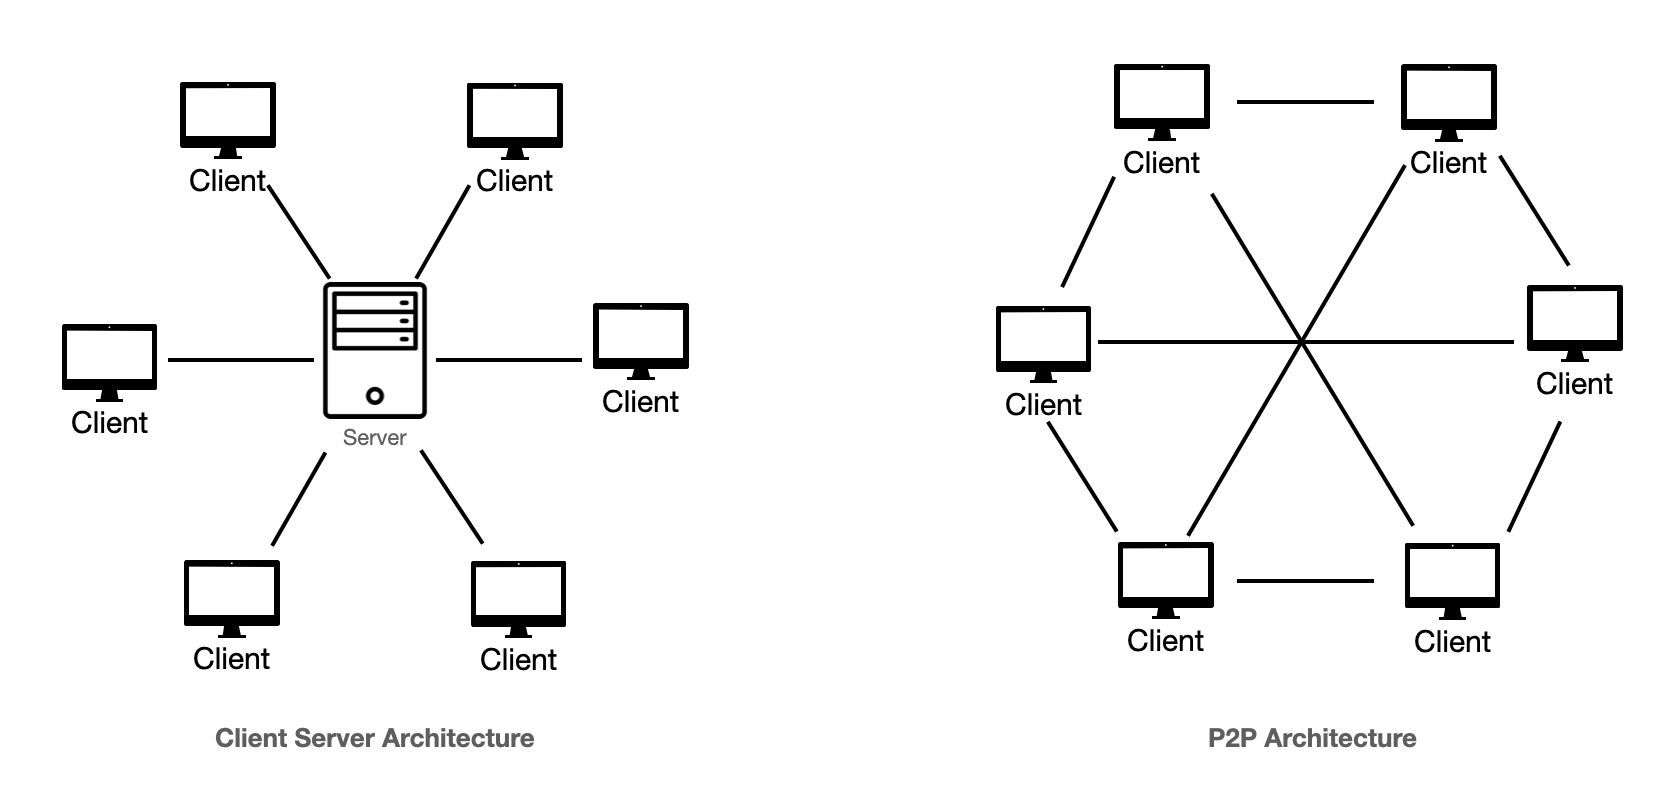
\includegraphics[width=12cm,height=6cm]{Images/Chap1/client-server-vs-p2p.png}
    \caption[Client-Server Architecture and P2P Architecture compared.]{Client-Server Architecture and P2P Architecture compared.}
    \label{clientservervsp2p}
\end{figure}

\subsection{Structure of a Block}\label{block_structure}
To begin, we present a concise overview of the structure of an individual blockchain block. A block is divided into two distinct parts: the \textit{header} and the \textit{body}. The block \textit{header}, illustrated in Figure~\ref{block_structure_img}, consists of six fields that govern the block itself:

\begin{figure}[h]
    \centering
    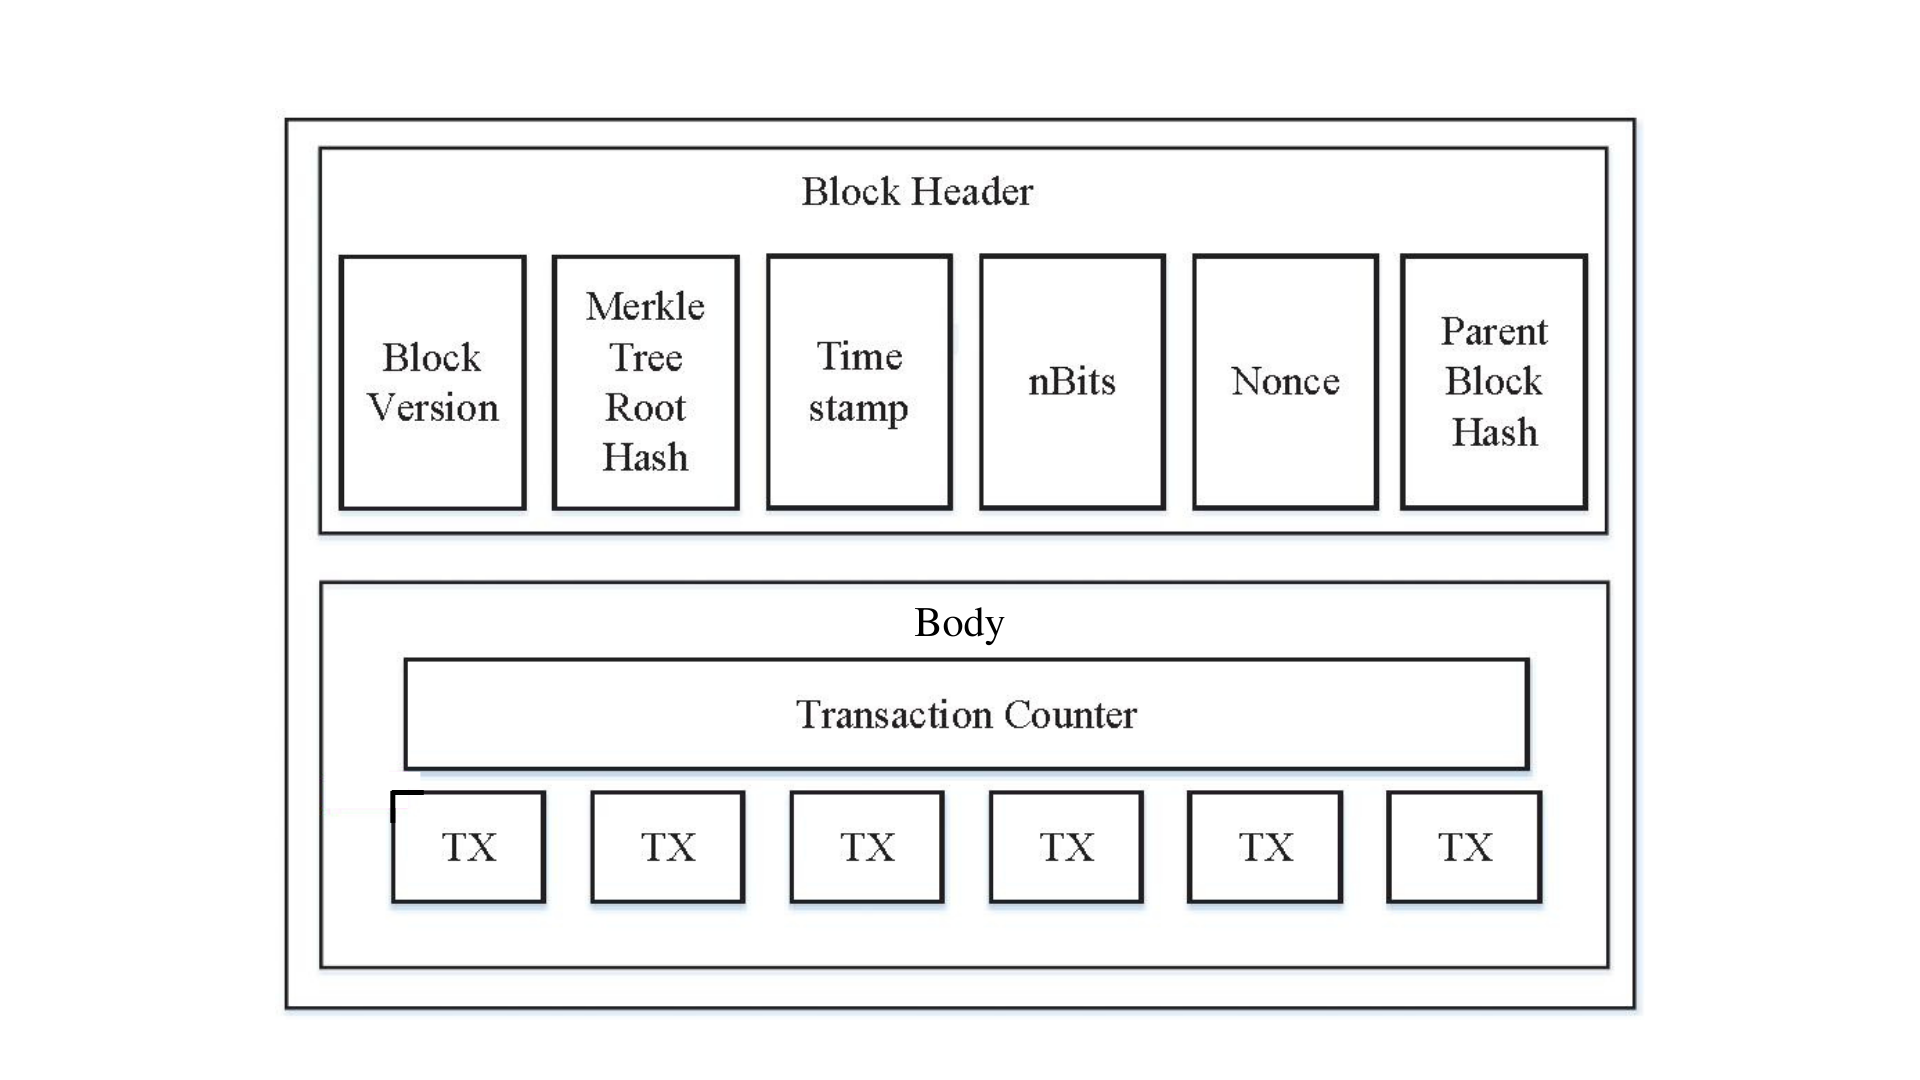
\includegraphics[width=14cm,height=7cm]{Images/Chap1/Block_Structure.png}
    \caption[Structure of a blockchain block]{Structure of a blockchain block.}
    \label{block_structure_img}
\end{figure}
\begin{itemize}
    \item \textbf{Version}: specifies the \textit{block‑validation rules}\footnote{Block validation is the essence of a blockchain. It allows the block to be appended to the chain only after a sequence of checks. }. The ruleset depends on the software version that drives the specific blockchain.

    \item \textbf{Parent Block Hash} (or \textbf{Previous Hash}): a 256‑bit value that references the preceding block in the chain. If the previous block's hash changes, so too does the \textit{Previous Hash}, triggering a cascade of updates across every subsequent block. See Section~\ref{hashing}.
    \item \textbf{Merkle Tree Root Hash}: the root of a Merkle tree used, among other purposes, to guarantee data integrity via hashing (Section~\ref{Merkle_Tree}).
    \item \textbf{Timestamp}: the precise instant of block creation, certifying that the recorded events occurred at that moment.
    \item \textbf{Bits} (or \textbf{difficulty target}): the Proof‑of‑Work threshold that a valid block hash must not exceed.
    \item \textbf{Nonce}: a byte‑level value repeatedly re‑hashed\footnote{Re‑hashing denotes successive hashing operations on the evolving header.} until the resulting hash meets the difficulty criterion. This computationally expensive search constitutes the well‑known process of \textit{mining}.
\end{itemize}

The block \textit{body} consists of a \textit{transaction counter} and the transactions themselves (denoted “TX” in Figure~\ref{block_structure_img}). Each transaction must be \textit{verified}\footnote{Verification confirms the details of the transaction, including timestamp, amount, and participants.}. The verification logic is examined in Section~\ref{transazioni}.

\subsection{Hashing for Block Linking}\label{hashing}
\begin{figure}[h]
    \centering
    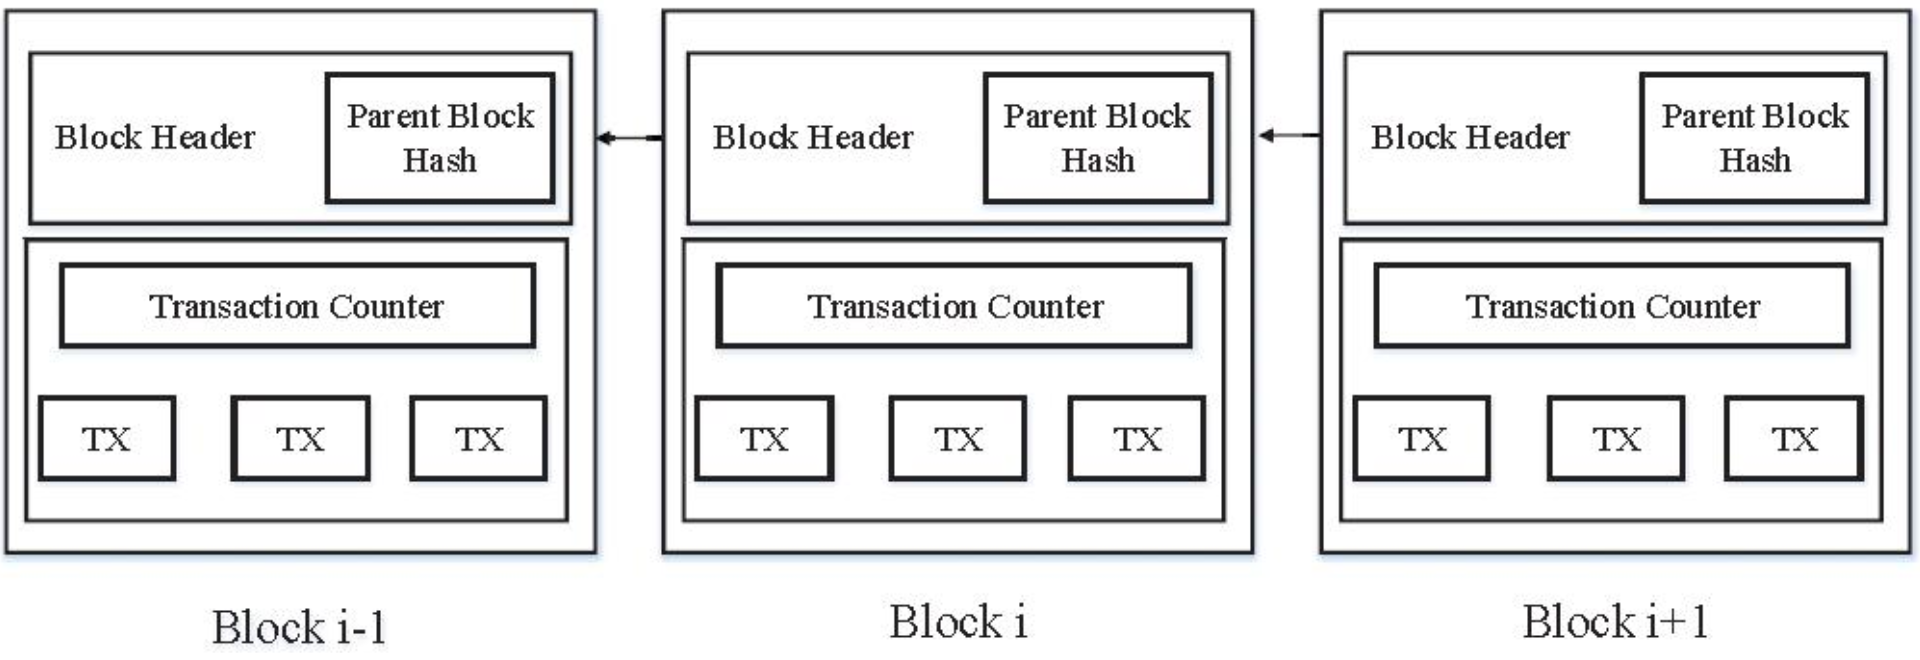
\includegraphics[width=12.5cm,height=5cm]{Images/Chap1/Chain.png}
    \caption[Minimal schematic of a blockchain]{Minimal schematic of a blockchain.}
    \label{chain_img}
\end{figure}
As noted above, a blockchain is a data structure composed of sequentially linked blocks (a minimal schematic appears in Figure~\ref{chain_img}). New blocks form whenever network participants create fresh data or update existing records. Each block stores cryptographically protected data together with a unique identifier: the block hash.

The hash is the adhesive that binds blocks together, producing a genuine \textit{chain of blocks}. By design, it renders the chain tamper‑evident, ensuring both the integrity and authenticity of every block's data. This subsection introduces hashing in general and its specific application in blockchain technology.

Hashing is the process whereby an arbitrary key $k$ is fed to a \textit{hash function} $h$ to obtain an integer $h(k)$. The key-value pair \lstinline|<k,v>| is stored in a vector (the \textit{hash table}) at position $h(k)$. Formally,
\begin{equation*}
    h : U \rightarrow \{0,1,\dots,m-1\}, \quad\text{where}
\end{equation*}
\begin{itemize}
    \item $h$ is the hash function;
    \item $U$ is the Universe set of possible keys;
    \item $m \in \mathbb{N}$ is the size of the vector $T$;
    \item $T$ is the hash table that stores the key-value pairs, exemplified in Figure~\ref{hash_table} as \textit{storage}.
\end{itemize}
\begin{figure}[h]
    \centering
    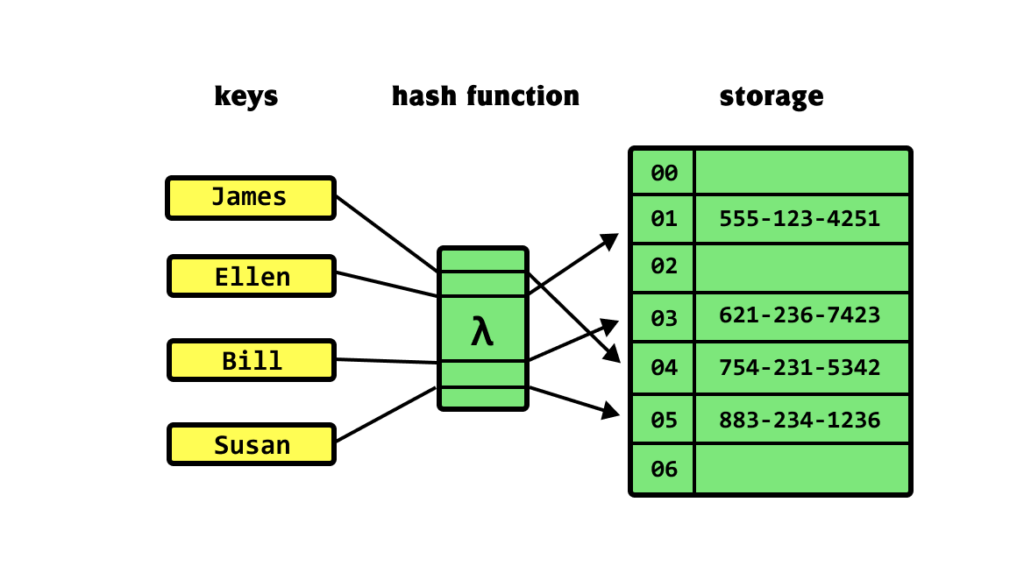
\includegraphics[width=12cm,height=7cm]{Images/Chap1/hash_function.png}
    \caption[Example of a hash table]{Example of a hash table.}
    \label{hash_table}
\end{figure}

Within a blockchain, \textit{cryptographic hash functions}, a specialized subset of classical hash functions, must satisfy the following properties:
\begin{itemize}
    \item \textit{Determinism}: identical input always yields the same hash.
    \item \textit{Collision resistance}: finding two distinct inputs that produce the same hash is computationally infeasible.
    \item \textit{Pre‑image resistance}: deriving the original message from its hash is computationally infeasible.
    \item \textit{Efficiency}: the hash must be computable quickly.
\end{itemize}
These attributes make cryptographic hash functions ideally suited to guarantee integrity, authenticity, and data security.

Applied to blockchain, the hash endows each block with uniqueness. Because every block includes the hash of its immediate predecessor, any alteration to a block propagates forward, invalidating all successors. As highlighted in Section~\ref{block_structure}, each block also contains a \textit{timestamp} that contributes to its hash and, in the words of \cite{bitcoin}, “[...] proves the data must have existed at that time, since it features in the hash.”

There are numerous cryptographic hash functions, but over time, it has been shown that some of them have vulnerabilities. Today, the most widely employed family is the \textit{Secure Hash Algorithm} (SHA). Collisions discovered in SHA‑0 and SHA‑1 render them ill‑advised for new deployments, whereas more recent variants remain robust. Bitcoin employs SHA‑256 (a SHA‑2 family member) with a 256‑bit digest. Ethereum, before \textit{The Merge} upgrade of 15 September, used Keccak‑256 with a variable‑length digest; Keccak is the basis for SHA‑3, the latest member of the SHA standard family.

\subsection{Public-key cryptography} \makeatletter\def\@currentlabel{Public-key cryptography}\makeatother
\label{pubkey}
In 1976, Whitfield Diffie and Martin Hellman, working in concert with Ralph Merkle, introduced the concept of public-key (asymmetric) cryptography\,\cite{AsymCrytt}.  
This revolutionary idea rests on mathematically linked pairs of keys (public and private key).

A \textit{private key} is a randomly generated secret value known only to its creator.  
It is used:
\begin{enumerate}[label=\textit{(\roman*)}]
 \item To decrypt any message that has been encrypted with the matching public key; 
 \item To generate a digital signature.
\end{enumerate}

Every \textit{private key} is associated with a unique \textit{public key}, a number that can be distributed without restriction.  
Anyone may employ the public key to encrypt information intended for the key-pair owner or to verify signatures produced with the private key.

Cryptocurrencies dispense with a central authority to oversee transactions, but this raises the challenge of establishing trust among users.  
Consensus protocols resolve that difficulty by compelling the network's nodes to agree on which transactions are valid and by ensuring that once recorded, they remain immutable. \textit{PoW} and \textit{PoS} consensus protocols are mentioned respectively in \ref{pow} and \ref{pos}.


\subsection{Transactions: The Digital Signatures Chain Mechanism}\label{transazioni}
In a blockchain, transactions exchange assets of any nature among two or more parties and must be broadcast to and subsequently stored by every network participant. Because the system is decentralised, any transaction enjoys the same significance as any other; hence, all nodes must verify its authenticity.

Satoshi Nakamoto proposes in \cite{bitcoin} a system of \textit{digital signatures}. Every peer‑to‑peer (P2P) node holds a \textit{public key} and a \textit{private key}:
\begin{itemize}
    \item The \textit{public key} (often denoted as an address) is visible to every network participant.
    \item The \textit{private key} is known only to its owner.
\end{itemize}
To implement the digital‑signature system, each emitted transaction is signed with the hash value (generated as described in Section~\ref{hashing}) and the sender's private key. The resulting output is broadcast across the network using the recipient's public key. Only the recipient can decrypt the message, as only they possess the matching private key, and thus can verify the digital signature.

Once authenticity has been established, we must consider how transactions are stored within blocks. They are chained together by the \textit{Digital Signatures Chain}; as \cite{bitcoin} puts it, “[...]each owner, when transferring the coin, signs a hash of the previous transaction and the public key of the next owner[...]”. The outcome is a genuine chain of transactions, stored inside every block; a graphical illustration appears in Figure~\ref{transaction_chain}.
\begin{figure}[h]
    \centering
    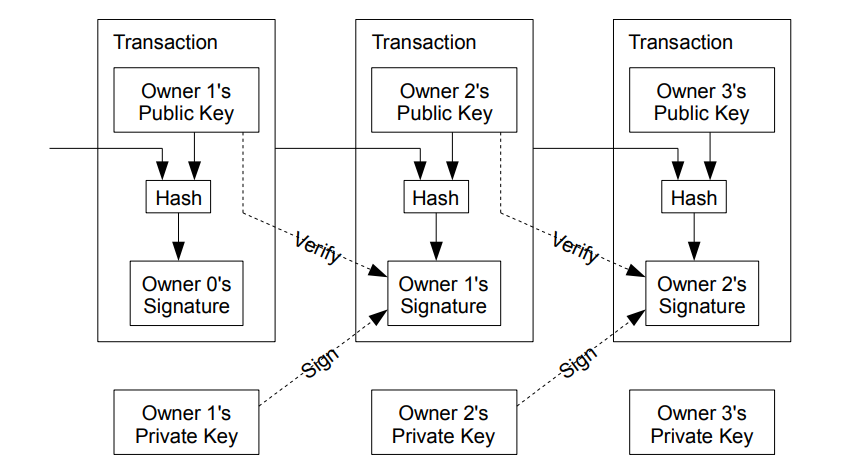
\includegraphics[width=12cm,height=7cm]{Images/Chap1/Transaction_Chain.png}
    \caption[Transaction Chain]{Transactions stored within a block via the Digital Signatures Chain mechanism.}
    \label{transaction_chain}
\end{figure}
As indicated in Section~\ref{block_structure}, multiple transactions reside in each block body. Each belongs to one or more transaction chains that collectively track the complete spending history of every participant's digital funds. In Bitcoin's white paper \cite{bitcoin}, the aggregated structure is termed \textit{electronic cash}.

\subsection{Merkle Tree Roots and Data Integrity}\label{Merkle_Tree}
A further component that guarantees data integrity within a block is the \textit{Merkle tree}, an \textit{arborescent} data structure\footnote{A tree is a data structure composed of nodes linked by edges, yielding hierarchical organisation.} whose single root (the Merkle Tree Root) is stored in the block header (see Section~\ref{block_structure}).

The bottom layer of this tree “[...]~displays the transactions stored (e.g.~T001 in Figure~\ref{merkle_root_img}), which are subsequently converted into their SHA‑256 hash digests (e.g.~H001), forming the leaves of the Merkle tree [...]” \cite{merkle_tree}.
\begin{figure}[h]
    \centering
    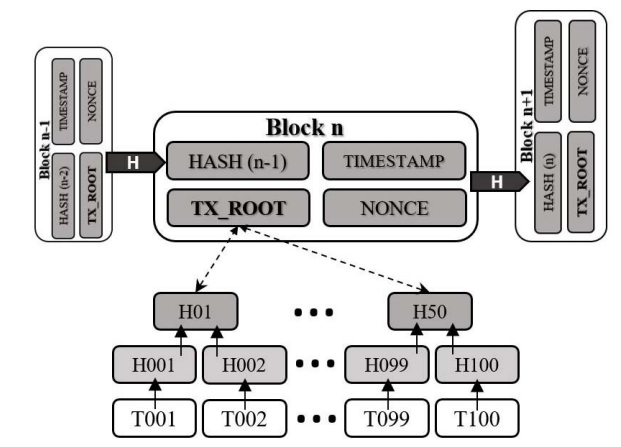
\includegraphics[width=12cm,height=8cm]{Images/Chap1/Merkle_Tree.png}
    \caption[Merkle Tree Root]{Merkle Tree Root stored in the block header.}
    \label{merkle_root_img}
\end{figure}
The root is computed by recursively hashing upward from the leaves. If even a single node is modified, the resulting hash variation propagates to the root, making any tampering immediately detectable. Consequently, nodes use the Merkle root to verify that received blocks are intact and that no past transaction has been altered.

\subsection{Proof‑of‑Work Mining for Block Validation}\label{pow}
Having understood transaction authenticity, we now examine how one or more transactions are \textit{validated}. Transactions must be broadcast to other network nodes for verification. In Bitcoin's mining model, specialised \textit{validator nodes} (\textit{miners}\footnote{Miners are owners of machines that contribute computational power and energy to a Proof‑of‑Work cryptocurrency network.}) receive the pool of pending, unvalidated transactions and propose the new block to be published.

To validate transactions and assemble them into a new block, miners must compute a specific value, the \textit{Nonce}, so that the resulting block hash satisfies a predetermined property. Recall that any change in the block's fields alters its hash. The computationally intensive task is precisely to adjust the Nonce until the hash meets the difficulty target.

Each block, together with its transaction history, must achieve a valid hash to be accepted. In Bitcoin, for instance, the criterion is that the block hash begins with a specific number of leading zeros. Only the first miner to solve the puzzle earns the block reward, a quantity of newly minted bitcoin generated by the process. Consequently, miners with greater computational resources enjoy a higher probability of capturing the reward.

Once mined, the block is appended to the blockchain, increasing its length, and all contained transactions are finalised.

\subsection{Proof‑of‑Stake Consensus for Block Validation}\label{pos}
In a Proof‑of‑Stake (PoS) system, the authority to extend the ledger derives from economic stake rather than raw computation, like in \ref{pow}. Prospective \textit{validators} lock coins in a deposit contract, exposing collateral that can be confiscated. As mentioned in \cite{validators}: “[...]~One validator is randomly selected to be a block proposer in every slot. This validator is responsible for creating a new block and sending it out to other nodes on the network. [...]”. The proposer assembles the pending transactions into a candidate block and broadcasts it together with a signature under her validator key; committee members independently verify the block and emit weighted attestations that are aggregated into its header.

Safety is underpinned by \textit{slashing}: any validator that equivocates or signs an invalid block forfeits a portion of its staked capital, turning misbehaviour into a direct financial loss. As long as two/thirds of the staked value adheres to the protocol, liveness and finality are preserved. The algorithm used in proof-of-stake Ethereum is called \textit{LMD-GHOST} \cite{buterin2020combiningghostcasper}, which overlays a longest chain rule with a Byzantine fault-tolerant voting gadget to deliver rapid, provable finality. Rewards sourced from transaction fees and, where applicable, inflationary issuance are apportioned among honest proposers and attesters, while penalties and opportunity costs disincentivise inactivity. Because consensus security is proportional to the value at stake rather than electricity expended, like in \textit{PoW}, \textit{PoS} drastically reduces energy consumption and lowers barriers to broad network participation.

\section{Bitcoin Overview}
\label{sec:bitcoin_overview}

Bitcoin went live in January 2009 with the \textit{genesis block}\footnote{Block 0 contains the newspaper headline “Chancellor on brink of second bailout for banks” from \textit{The Times} (3 Jan 2009). The line fixes the block date and alludes to the financial crisis. }.  The system introduced a public ledger secured by computation rather than by any central party.  Each transfer spends and creates \textit{unspent transaction outputs} (UTXOs); because every input must point to an existing, unspent output, the ledger forms an acyclic graph that auditors can follow to verify supply, as shown in Figure~\ref{utxos}.

\begin{figure}[h]
    \centering
    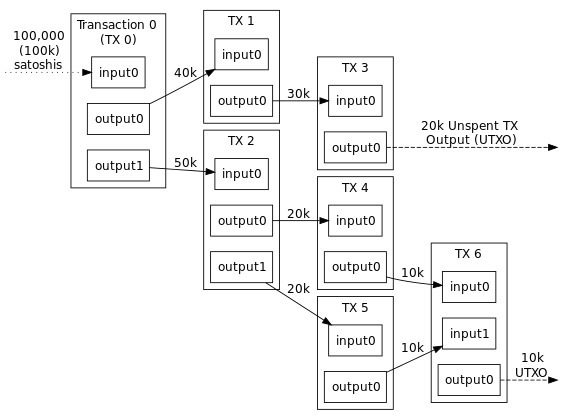
\includegraphics[width=10cm,height=6cm]{Images/Chap1/utxos.jpg}
    \caption[UTXOs]{UTXOs as used by Bitcoin. \cite{utxos}}
    \label{utxos}
\end{figure}

Time ordering relies on Proof-of-Work mining, outlined in Section~\ref{pow}.  Miners search for a block header whose double SHA-256 digest from Section~\ref{hashing} falls below the current target.  Nodes accept the chain with the greatest accumulated work, so an attacker would need to control nearly half of the global hash rate to rewrite history.

New coins enter circulation through the block subsidy.  The reward began at 50 BTC and drops by half every 210,000 blocks (halving \footnote{Procedure that halves by 50\% the creation of new Bitcoins every 210000 mined blocks (about every 4 years
considering that the mining time for the single block is 10 minutes).}), placing a hard limit of 21 million BTC on total supply. The calculation for reaching max supply is shown below.

\begin{equation*}
\sum\limits_{i=0}^{32}  210000 \cdot \frac{50}{2^i}       ,dove:
\end{equation*}

\begin{itemize}
\item The variable \textit{i} denotes the halving index, starting from zero and increasing up to the 32 halvings projected for the future.
\item \textit{210000} is the number of blocks that must be mined before the next halving occurs, and \textit{i} is incremented.
\item The value \textit{50} is the initial block reward in BTC; this amount is divided by $2^{i}$ at the \textit{i}-th halving.
\end{itemize}


Figure~\ref{btc_supply} illustrates how Bitcoin's total supply grows while the inflation rate steadily declines.

Bitcoin can handle about seven transactions each second because blocks arrive every ten minutes, and their size is small. Systems such as the Lightning Network move most payments off-chain and settle only the final balance on the main chain \cite{PoonDryja}. Projects like sidechains, merge-mined extensions, and covenants add extra tools around Bitcoin, but they still depend on its limited scripting rules. Privacy faces the same limits. Addresses hide names (pseudonymity), but not for long because cluster analysis often links them together \cite{Moser2013}.

After more than fifteen years online, Bitcoin is still a solid reference point for open settlement networks. Directly or indirectly, the idea of Bitcoin has contributed, and continues to contribute, to the development of new innovative solutions in the Web3 landscape.

\begin{figure}[h]
    \centering
    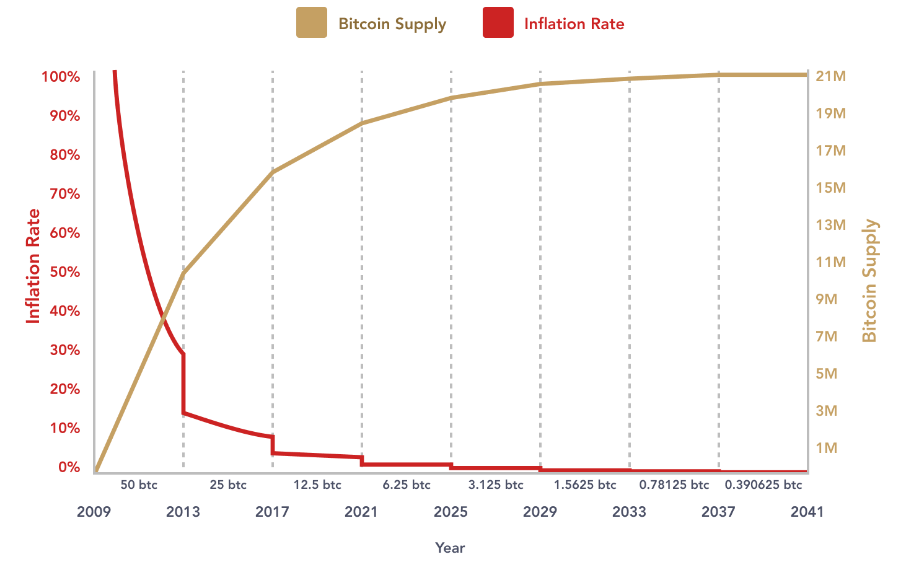
\includegraphics[width=12cm,height=6cm]{Images/Chap1/halving.png}
    \caption[Bitcoin issuance curve]{Cumulative bitcoin in circulation as block height increases.}
    \label{btc_supply}
\end{figure}

\section{Ethereum Overview}\label{ethOverview}

While Bitcoin spearheaded decentralized digital currency, Ethereum broadened these principles by providing a programmable blockchain equipped for diverse use cases. Conceived by Vitalik Buterin in 2014 \cite{ethereum}, Ethereum introduced \textit{smart-contracts}, which are self-executing programs embedded on the blockchain that automatically perform predefined conditions. The idea behind Ethereum is to create a large decentralized system, which goes beyond being a simple means of payment or a way to transfer money, but also a structure that can be programmed into everything from the automation of monetary exchanges to actual decentralized applications.

At the heart of Ethereum is the Ethereum Virtual Machine (EVM), a universal environment that ensures consistent execution of smart contract code across all nodes in the network. This unifying approach fosters robust security and facilitates a wide array of possibilities, ranging from finance, with decentralized finance (DeFi), to gaming and digital identities. Since introducing a Turing-complete virtual machine in 2015, Ethereum, with its EVM, has transcended simple peer-to-peer payments to become a programmable settlement layer, serving as a foundation for advanced, decentralized ecosystems.

The next subsections will explain the key components of Ethereum that matter for a zero-knowledge exploit platform such as \textit{zkpoex}.  The focus is on the account model, the EVM execution flow, the compilation toolchain, and smart contracts.

\subsection{Account Model: Externally Owned Accounts vs.\ Contract Accounts}\label{subsec:accounts}

Ethereum keeps state in a modified Merkle Patricia tree whose leaves are \textit{accounts}.  
Two categories exist:

\begin{itemize}
  \item \textbf{Externally Owned Accounts (EOA):}  Identified by a public key hash, they hold a \textit{balance} and a \textit{nonce}.  They cannot store bytecode and act only via signed transactions.
  \item \textbf{Contract Accounts:}  They embed immutable bytecode and point to a storage trie.  Code is executed when the account receives a \texttt{CALL} or \texttt{CREATE}.  
\end{itemize}

Each account node stores four fields: \textit{nonce}, \textit{balance}, \textit{storageRoot} and \textit{codeHash} \cite{Wood2014}.  
Figure~\ref{fig:account_model} shows the high-level layout.

The separation of signature logic (EOAs) from execution logic (contracts) is central to exploit proofs: \textit{zkpoex} emulates an EOA that triggers a vulnerable contract and then proves the resulting state transition without revealing the payload.

\begin{figure}[h]
  \centering
  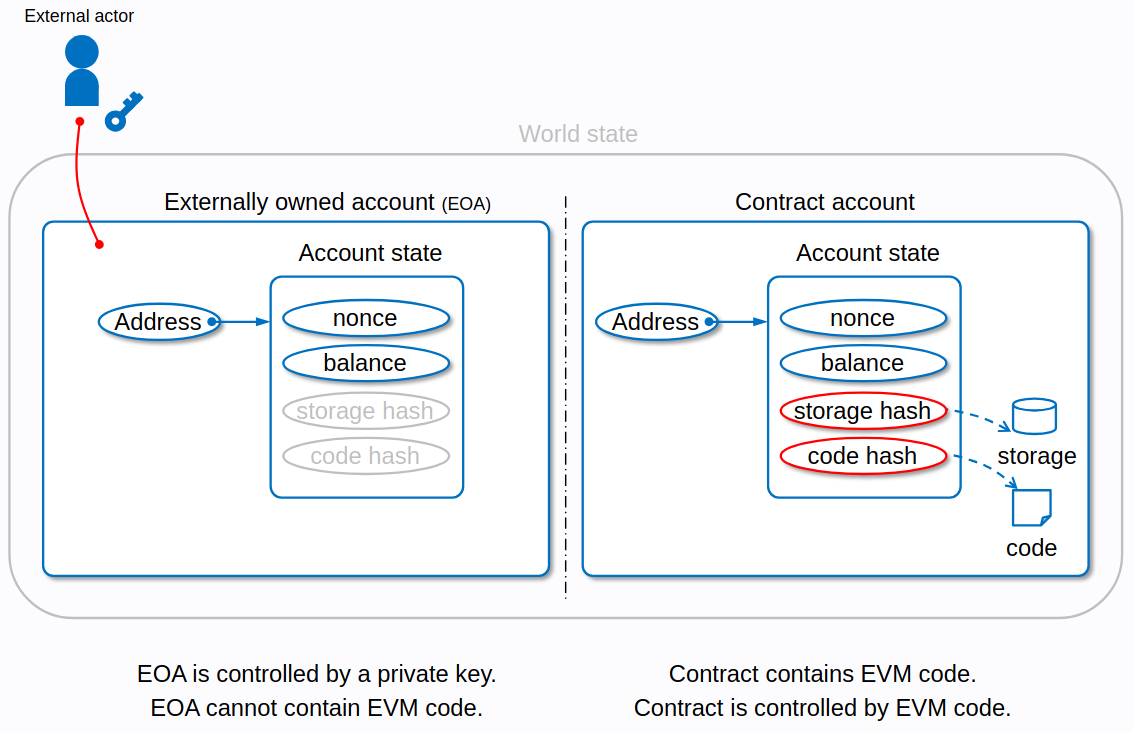
\includegraphics[width=12cm,height=8cm]{Images/Chap1/account_model.png}
  \caption{Ethereum account structure and differences between EOAs and contract accounts. \cite{ethacccounts}\cite{pdfEthAccounts}}
  \label{fig:account_model}
\end{figure}

\subsection{Transactions and Gas Accounting}\label{subsec:tx_gas}

Ethereum recognises several transaction formats, all wrapped in the \textit{typed-transaction envelope} introduced by \texttt{EIP-2718}.\cite{EIP2718}  
The most common types are:

\begin{enumerate}
  \item \textbf{Legacy (type~0):}  Fields are \textit{nonce}, \textit{gasPrice}, \textit{gasLimit}, \textit{to}, \textit{value}, \textit{data}, and the signature triple $(v,r,s)$.\cite{Wood2014}
  \item \textbf{Access List (type~1):}  Adds an \textit{accessList} array that pre-declares storage keys to lower the dynamic gas cost.\cite{EIP2930}
  \item \textbf{Dynamic Fee (type~2):}  Replaces \textit{gasPrice} with \textit{maxFeePerGas} and \textit{maxPriorityFeePerGas}.  The base fee is burned, and only the priority fee rewards the validator.\cite{EIP1559}
\end{enumerate}

The prototype detailed in this thesis limits its analysis to \textbf{legacy (type 0) transactions}.  
By working with a single, stable encoding, the prover avoids access-list handling (for type 2 txs) and the dynamic base-fee logic of post-London blocks (for type 3 txs).  
This simplifies byte stream parsing inside the \texttt{Risc0} zkVM and keeps on-chain verification compact.



\subsubsection{Construction and Broadcast}  
A user assembles the transaction, signs the RLP\footnote{RLP is a data encoding scheme used to serialize objects into a space-efficient binary format, particularly for transactions and other data structures.}-encoded payload, and submits it to the P2P network. Each node verifies the signature, checks that \textit{nonce} matches the sender's account counter, and computes the \textit{intrinsic gas} $g_0$:

\[
g_0 =
g_\text{tx} +
g_\text{data\_zero}\,\times\,n_\text{zero} +
g_\text{data\_nonzero}\,\times\,n_\text{nonzero} +
g_\text{accesslist}\,\times\,n_\text{access}
\]

as defined in Appendix~G of the Yellow Paper.\cite{Wood2014}  
The transaction is rejected if $g_0 > \textit{gasLimit}$.

\subsubsection{Mempool and Inclusion}\label{sssec:mempool}
Once a node validates a signed payload, it places the transaction in its
\textit{mempool} a local priority queue shared with peers. Every block
builder repeatedly scans this pool, sorting candidates by the \textit{effective
fee}:

\[
\text{effFee}
= \min\!\bigl(\textit{maxFeePerGas},\;
              \text{baseFee} + \textit{maxPriorityFeePerGas}\bigr),
\]

then fills the next block with the most profitable bundle that fits beneath
the block‐gas target.  The flow from wallet to on-chain inclusion is sketched
in Figure~\ref{fig:tx_flow}.  After \texttt{EIP-1559}, the single
\textit{gasPrice} field is split into two: an \textbf{algorithmic base fee}, burned
by the protocol to balance demand, and an optional \textbf{tip} that rewards
validators for fast service.

\begin{figure}[h]
  \centering
  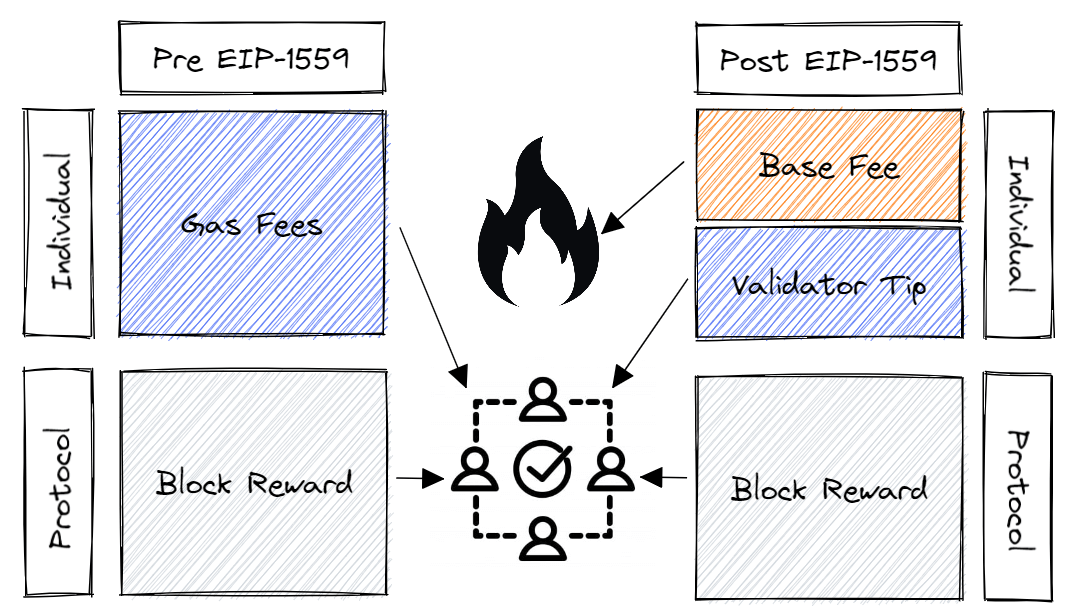
\includegraphics[width=.85\linewidth]{Images/Chap1/eip1559.png}
  \caption{Fee mechanics before and after \texttt{EIP-1559}.\cite{londonFork}}
  \label{fig:tx_flow}
\end{figure}

\subsubsection{Execution and Settlement}
At block time, the EVM executes transactions in the chosen order, deducting \textit{intrinsic gas} up-front and consuming the remaining budget opcode by opcode. If gas is exhausted, the call reverts, state changes in that call frame are discarded, yet the gas already spent stays with the validator.  Whenever execution finishes successfully, any unused gas is refunded to the sender, subject to the usual \(\text{gasRefund}\le\frac12\text{ gasUsed}\) cap, and logs are appended to the block receipt trie. The final state root, transaction root, and receipt root are then committed in the block header, making the result immutable.

\subsection{Smart Contracts on Ethereum}\label{subsec:smart_contracts}

Smart contracts are self-contained programs deployed directly on the Ethereum blockchain. Once a contract’s bytecode is published through a \texttt{CREATE} transaction, every full node executes the same immutable code whenever a subsequent call targets the contract address, guaranteeing that all participants observe an identical state transition. In practice, these on-chain programs behave like autonomous “digital vending machines”: given a valid transaction carrying the correct function selector and arguments, they automatically transfer funds, update storage, or emit events, requiring no intermediary.

\texttt{Solidity} is the de facto language for writing such contracts and is therefore the language chosen for \textit{all} vulnerable case studies in this thesis.  

Its popularity brings three concrete advantages:
\begin{enumerate}
    \item \textbf{Dominant footprint}: the vast majority of on-chain applications, audits, and public exploit reports are written in Solidity so that researchers can reuse known patterns without a steep learning curve.
    \item \textbf{Mature tooling}: frameworks such as Hardhat, Foundry, Slither, and Echidna streamline compilation, testing, and static analysis.
    \item \textbf{Direct EVM target}: the Solidity compiler outputs raw EVM bytecode, meaning an exploit written in Solidity exercises exactly the same low-level execution paths that \textit{zkpoex} will replay and prove inside the RISC Zero zkVM.
\end{enumerate}

By building on Solidity’s rich ecosystem, \textit{zkpoex} significantly improves the handling of smart contract bytecode and state transitions. Leveraging \texttt{solc}\footnote{\texttt{solc} is the official command-line compiler for Solidity; it turns \texttt{.sol} source files into EVM bytecode and ABI description in a single step.}, developers can compile existing exploit proofs-of-concept into actual runtime bytecode, automatically extract ABI, bytecode, metadata, perform library linking, and target specific EVM versions. As a result, there is no need to manually reconstruct EVM traces or simulate low-level behavior. Instead, the exact binary generated by \texttt{solc} becomes the input to \textit{zkpoex}, which feeds it into the zkVM for zero-knowledge proof generation.


\section{Zero-Knowledge Proofs (ZKPs)}\label{zkpChap}
Zero-knowledge proofs (ZKPs) appear to be an innovative solution to ensure privacy and security in various digital interactions. By allowing a party to demonstrate knowledge of a fact without revealing any additional information, ZKPs offer a powerful tool for building trust in systems where confidentiality is paramount. This capability has significant implications in fields such as secure communications, authentication, and blockchain technologies. In the following sections, we will elaborate the key concepts underlying ZKPs, provide the historical context for their development, and explore very simple illustrative examples to clarify their mechanism. Through this exploration, we will delve deeper into how ZKPs work and their importance in modern cryptographic practices.

\subsection{History of ZKPs}\label{zkHistory}

In 1985, the foundational idea of zero-knowledge proofs (ZKPs) was introduced in a peer-reviewed academic paper titled “The Knowledge Complexity of Interactive Proof Systems”\cite{MITzkstudy}. This work represented a significant advancement in the field of cryptography, authored by researchers Shafi Goldwasser, Silvio Micali, and Charles Rackoff from MIT.

According to the author's description, the original idea involved “\textit{interactive protocols}”, in which the prover and verifier would repeatedly communicate in order to persuade the verifier that the prover was correct.  Despite being a breakthrough in its own right, this method was time and resource-intensive, especially when dealing with large amounts of data.  Zero-knowledge proofs must not be interactive in order to be \textit{scalable}.

In 1986, Amos Fiat and Adi Shamir showed that the interaction in many public-coin zero-knowledge proofs could be eliminated by replacing the verifier's random challenge with the output of a publicly available hash function, an idea now known as the \textit{Fiat–Shamir heuristic} \cite{fiatShamirHeuristic}.  Their transformation converts an identification protocol into a digital-signature scheme and, more broadly, turns an interactive proof of knowledge into a \textit{non-interactive zero-knowledge} (NIZK) proof.  Because no live exchange is required, the resulting proofs are ideally suited to settings, such as online transactions or blockchains, where prover and verifier cannot communicate in real time.

Two years later, Manuel Blum, Paul Feldman, and Silvio Micali provided the first \textit{formal} framework for NIZK by introducing the \textit{common reference string} (CRS) model \cite{blumFeldmanMicali1988}.  They proved that, given a short random string shared in advance, every language in \textit{NP} admits a computational zero-knowledge proof with no interaction, thereby establishing the theoretical generality of NIZKs beyond the random oracle setting assumed by Fiat and Shamir. Illustrative figure in \ref{fig:zkpvsnizkp}.

After a few years, the next push toward ZKPs occurred in 2011, when Nir Bitansky, Ran Canetti, and Alessandro Chiesa published a paper at the International Symposium on Theory of Cryptography titled “\textit{From extractable collision resistance to succinct non-interactive arguments of knowledge, and back again.}”\cite{zksnark}.
This study demonstrated how to generate \textit{SNARKS} (succinct non-interactive arguments of knowledge) using a function known as the \textit{Extractable Collision Resistance (ECR)} hash function.  In essence, SNARKS are ZKPs that are “succinct”, which means they are small in size and can be verified in a few seconds.

\begin{figure}[h]
    \centering
    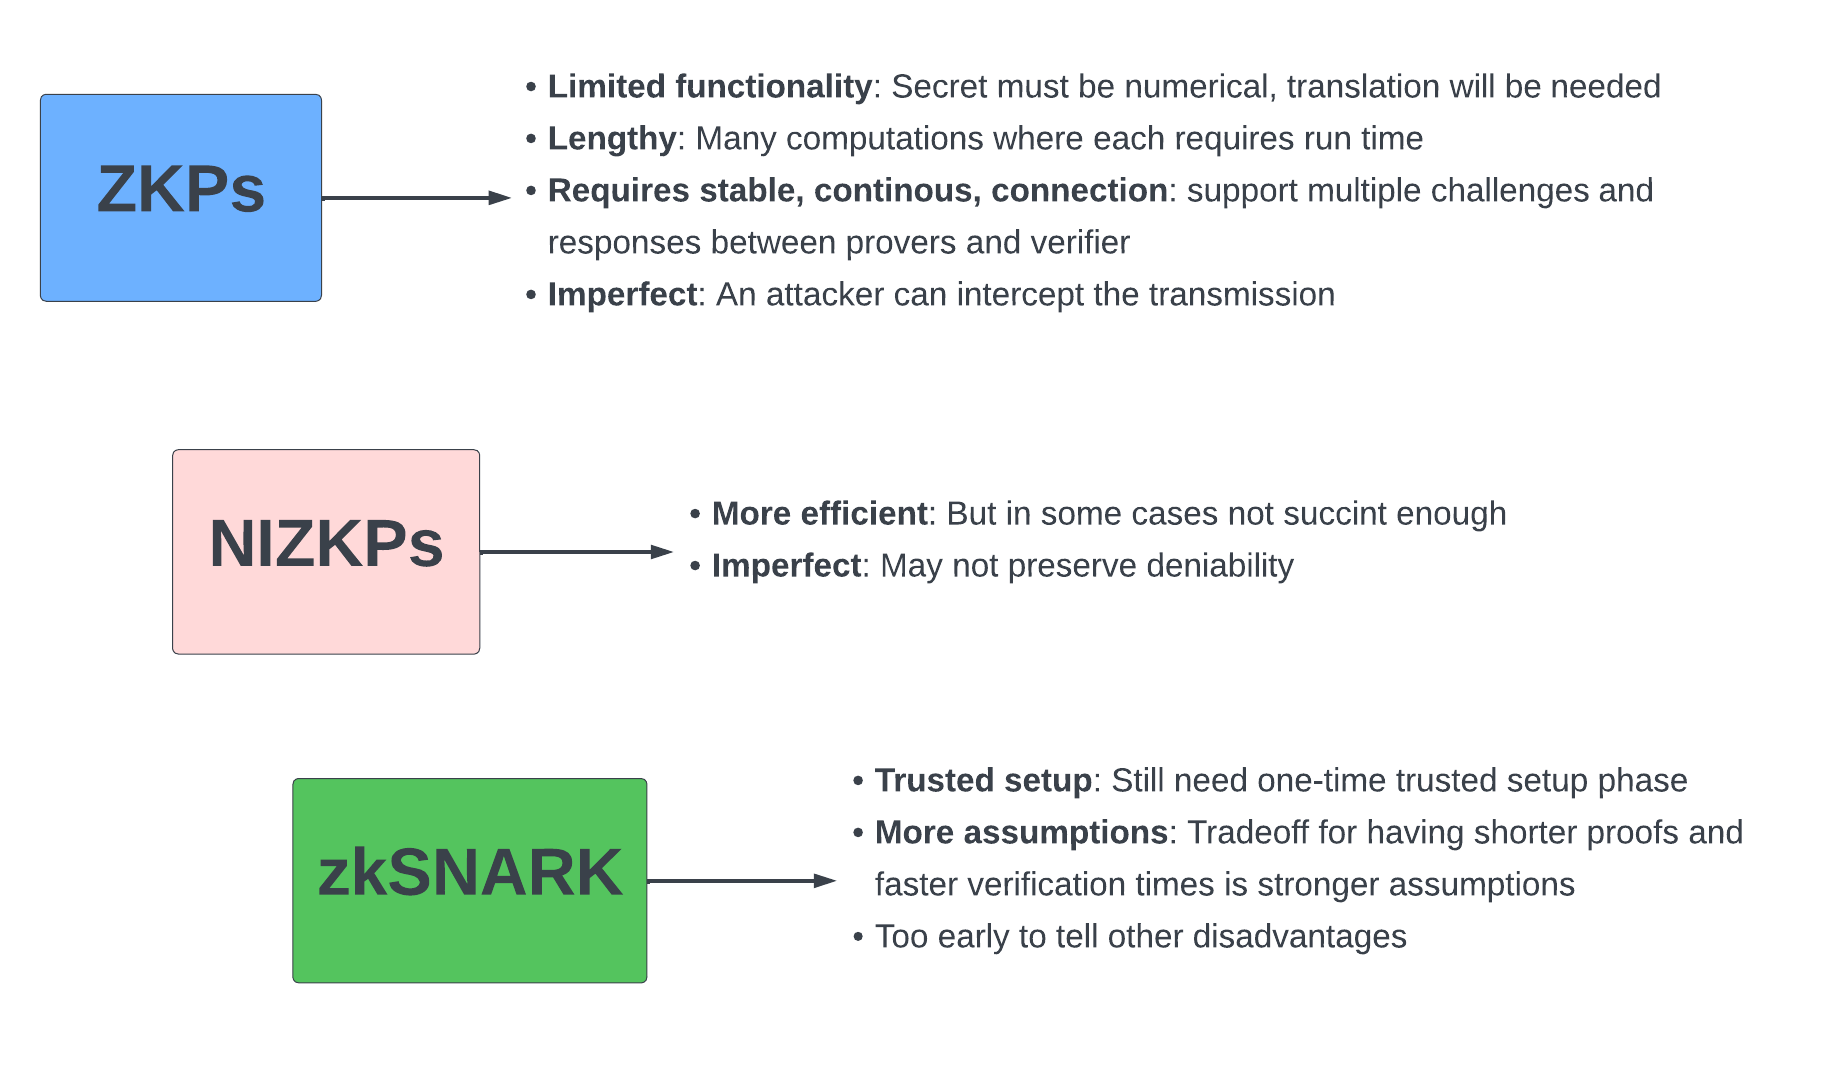
\includegraphics[width=1\linewidth]{Images/Chap1/comparisionZK.png}
    \caption{A comparison of ZKPs, NIZKPs and zk-SNARKs \cite{zkcamp}}
    \label{fig:zkpvsnizkp}
\end{figure}

Despite the verification speed and scalability of zk-SNARKs, some implementations, such as \textit{Pinocchio}\cite{pinocchio}, had some limitations:
\begin{itemize}
    \item \textbf{Trusted setup:}  Classical zk-SNARKs begin with a one-off “\textit{ceremony}” that produces public parameters for everyone to use.  The people running this ritual briefly handle secret randomness, often called \textit{toxic waste}, which must be destroyed.  If even one participant kept a copy, they could later forge convincing proofs, so the whole system inherits a small but real point of trust. An illustration can be seen in Figure \ref{fig:trustedSetup}.
    \item \textbf{Not post-quantum secure:}  These proofs lean on hardness assumptions such as the elliptic-curve discrete-log problem.  A large-scale quantum computer could solve that problem efficiently, undermining cryptography and allowing forged proofs.
\end{itemize}

\begin{figure}[h]
    \centering
    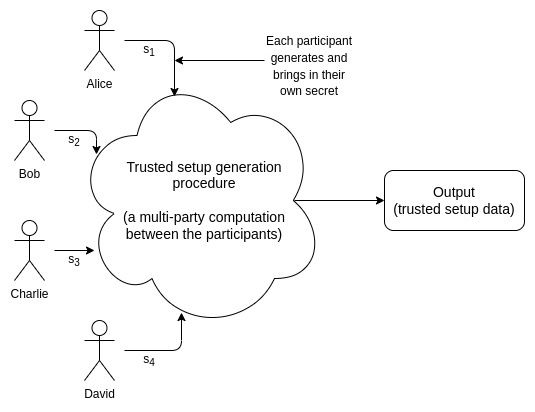
\includegraphics[width=0.9\linewidth]{Images/Chap1/trusted_setup.png}
    \caption{A trusted setup ceremony procedure, where \textit{s} are all secrets.\cite{vitalikblogTrustedSetup}}
    \label{fig:trustedSetup}
\end{figure}

From this moment on, the development of ZKPs accelerates greatly. Indeed, only two years later, in 2016, Jens Groth showed that zk-SNARKs could be both short and fast.
His construction, now simply called \textit{Groth16}, as shown in the paper “\textit{On the Size of Pairing-based Non-interactive Arguments}”\cite{groth16}, shrinks the public parameters and the proof itself to just three curve points each.
Verification is reduced to a handful of pairings that finish in milliseconds on a laptop, while the proof fits in roughly two hundred bytes. The performance leap was so large that privacy-oriented blockchains such as Zcash\footnote{Cryptocurrency that focuses on privacy and anonymity, offering users the option of both transparent and shielded transactions.} adopted Groth16 almost immediately, and a thriving ecosystem of circuit compilers, libraries, and auditing tools has formed around it. It is still being used in a lot of protocols today, like the one on which the software of this thesis was developed: Risc0. 
As will be discussed in more detail in Section \ref{proof_system}, Risc0 uses a “STARK-to-SNARK” circuit, and as a SNARK, it uses precisely \textit{Groth16}.



The next wave arrived in 2017 with \textit{Bulletproofs} by Bünz, Bootle \textit{et al.},\cite{bulletproof}.
Bulletproofs are logarithmic-length, non-interactive proofs that rely only on the discrete log assumption, so they dispense entirely with the trusted setup.
Their flagship feature is the \textit{range proof}: one can convince a verifier that an encrypted value falls inside a chosen interval without revealing the value itself.
Many such statements can be aggregated into a single short proof, keeping confidential transactions on Bitcoin-style chains small enough for everyday use.
The absence of toxic waste, combined with good practical performance, made Bulletproofs an instant favourite in “trustless” blockchain design.

Together, Groth16 and Bulletproofs reshaped the field: the former proved that zk-SNARKs could be truly lightweight, while the latter showed that trusted ceremonies are not a necessity.
Their success paved the way for the flurry of post-2018 research into transparent, post-quantum-ready proof systems and the recursive techniques that power today's layer 2\footnote{Second-layer (off-chain or partially off-chain) scalability protocols that periodically commit their state to the main blockchain. } scalability solutions. 
The spotlight then shifted in 2018 when Ben Sasson \textit{et al.} introduced zk-STARKs, \textit{Zero Knowledge Scalable Transparent ARguments of Knowledge}, which swap pairing based cryptography for hash based commitments and replace the one off ceremony with a public randomness beacon, making the system both post quantum resilient and fully transparent\cite{benSassonSTARK2018}. 

Although the resulting proofs are noticeably larger, often running to tens or even hundreds of kilobytes, the design proved that trusted setup is not a law of nature and sparked a race to shrink proof sizes without reintroducing toxic waste.  PLONK\footnote{Polynomial Commitment scheme over Lagrange bases for Non-interactive arguments of Knowledge.} followed in 2019: by adopting a universal, updatable structured reference string, it slashes the number of ceremonies to one, and that ceremony can be refreshed at will, thus reducing the trust footprint while sustaining Groth16 level efficiency\cite{gabizonPlonk2019}.  In parallel, Bowe, Grigg, and Hopwood unveiled \textit{Halo}, showing that recursive composition is possible in the discrete log world without any setup at all; their technique allows unlimited proof aggregation and laid the groundwork for succinct block verification\cite{boweHalo2019}.  Recursion soon became leaner still: Setty's \textit{Nova} (2021) introduces a folding scheme whose verifier costs only a handful of group operations and whose prover needs no FFTs\footnote{Fast Fourier Transforms: algorithms that compute discrete Fourier transforms in \(O(n\log n)\) time and are heavily used in polynomial-based proof systems.} or ceremony\cite{settyNova2021}.  The fold and aggregate idea has since been generalised by protocols such as \textit{Protostar} and \textit{HyperNova} (2023), which support high-degree gates, lookups, and other features required by modern zk virtual machines\cite{bunzProtostar2023}.  Industry deployments kept pace: Polygon's \textit{Plonky2} (2022) marries STARK-style arithmetisation with PLONK-inspired recursion, producing millisecond-scale proofs on consumer hardware and powering roll-ups like Polygon zkEVM\cite{polygonPlonky2Blog2022}. By 2024/25, the ecosystem has converged on hybrid stacks, fast STARK proofs compressed by compact SNARK wrappers, running on GPU- and VPU-accelerated hardware; a recent survey lists more than twenty open-source frameworks that developers can benchmark out-of-the-box \cite{sheybaniZKPSurvey2025}.  
Building on these hybrid foundations, in May 2025, StarkWare unveiled \textit{Stwo}, a next-generation open-source STARK prover written in Rust that implements the new Circle STARK protocol \cite{circleSTARK}.  
Early benchmarks exceed 500 k-hash/s on a commodity quad-core laptop\footnote{“Hash/s” counts the Keccak/Fri-hash evaluations that dominate STARK proving time. At 500 000 hash/s, a 2 M-hash roll-up circuit completes in roughly four seconds; first-generation STARK prototypes (in 2018) achieved below 5 000 hash/s on similar hardware, pushing the same circuit well past the ten-minute mark.}, and a WebAssembly build has already demonstrated full client-side proving directly in the browser: the first time complete proofs can be generated and verified on off-the-shelf devices.  
\textit{Stwo} combines aggressive arithmetic optimisations with a modular design slated for Starknet's production stack, paving the way for web-scale, on-device proof generation.  
In less than a decade, zero-knowledge proofs have evolved from megabyte-scale, ceremony-bound prototypes to sub-kilobyte, post-quantum-ready proofs that settle blockchain state every few seconds, and the trajectory suggests that constant-time, constant-memory ZKPs are now within realistic reach of 2030-era devices.

\subsection{Illustrative examples of ZKPs} \label{zkExamples}
ZKPs are often a very complicated concept to understand, so to visualize this idea easily, we will present two famous abstract examples.
\subsubsection{The Ali Baba Cave} \label{AliBabaCave}

The first example we will discuss was first exposed in \cite{howtoexplainzk}, it offers a particular insight into how protocols using zero-knowledge proofs operate. Picture Ali Baba, an elderly merchant from Baghdad, who visits the bazaar daily to trade goods. One day, a thief grabbed a purse from Ali Baba and fled into a uniquely shaped cave. Upon reaching the cave, Ali Baba encountered two dark, winding passages: one to the left and the other to the right. Having missed which way the thief went, he was compelled to make a choice. After a moment of contemplation, he decided to investigate the right passage. Unfortunately, he found no sign of the thief, only to reach a dead end. Concluding that the thief might have taken the other passage, he ventured left, but again found nothing; that route also led to a dead end.
Disheartened, Ali Baba realized the thief had likely escaped while he was still in the first passage. Sad about his loss, he returned home and went to sleep. The next day, as Ali Baba made his way back to the bazaar, another thief grabbed Ali Baba's basket and headed for the same cave. Once more, Ali Baba faced the same dilemma. 

\begin{figure}[h]
    \centering
    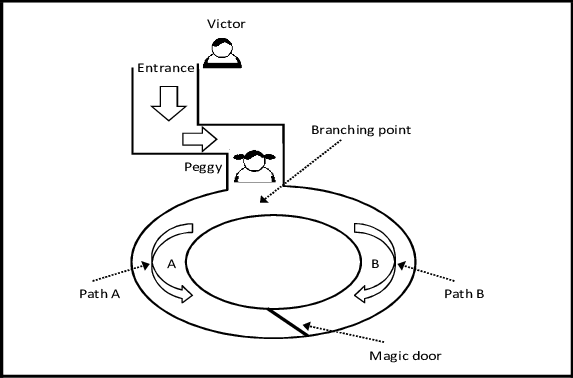
\includegraphics[width=0.7\linewidth]{Images/Chap1/alibaba.png}
    \caption{Ali Baba's cave representation.}
    \label{fig:alibaba}
\end{figure}


As the days passed, Ali Baba found himself repeatedly robbed by a thief who always escaped into the cave, leaving him frustrated and confused. Each time, he convinced himself that luck favored the thieves, allowing them to choose the passage he hadn't selected. However, on the fortieth day, after being robbed for the fortieth time, Ali Baba began to suspect that the cave concealed a significant secret. Determined to uncover the truth, he decided to hide in one of the dark passages and wait for a thief to reach a dead end. Hours went by, and finally, a thief rushed through the passage. Spotting another merchant behind him, the thief uttered the magical words, “Open sesame.” To Ali Baba's surprise, a hidden entrance in the wall of the dead end slid open, allowing the thief to slip through and close the passage behind him. Ali Baba realized that the right passage was connected to the left one when the wall moved. Intrigued, he spent a long time experimenting with the magic words, eventually modifying them as if he were changing the code on a lock. The next day, when a thief attempted to rob him again, Ali Baba was ready and managed to trap him, preventing any escape. He recorded this experience in an illustrated manuscript, but he deliberately omitted the new magic words, leaving behind subtle hints for anyone clever enough to discover them. Years later, a researcher stumbled upon the manuscript and deciphered the magic words. Excited by this revelation, he invited a group of reporters to the cave to witness his discovery, but he cleverly withheld the actual magic words from them. How did he manage this? The process was straightforward. First, a television crew filmed an extensive tour of the cave, capturing the two dead ends, before leaving. The researcher then re-entered the cave through one of the passages. Following him, the reporter, with a camera in tow, entered and reached the fork in the path, where he flipped a coin.
\begin{itemize}
    \item If the coin landed heads, he would instruct the researcher to exit from the left.
    \item If it landed tails, he would signal for the researcher to come out from the right.
\end{itemize}
    
The researcher would then emerge from whichever direction the reporter indicated. This procedure was repeated 40 times, commemorating the same number of times Ali Baba had been robbed. Each repetition cut the probability of the researcher emerging from the correct passage in half, leading observers to believe he must have known the secret words after consistently appearing from the designated exit.
Now we arrive at the intriguing part of the tale. After the original tape was recorded, another reporter sought to tell this remarkable story, but the researcher refused to cooperate. In a twist of mischief, he instead disclosed the cave's location to the envious reporter. This reporter hired an actor resembling the researcher and returned to the cave to replicate the earlier recording. However, this time the actor was unaware of the magic words. Each time he exited the wrong passage, the reporter edited the footage, cutting those segments and repeating the process until the coin flip aligned with the actor's exit. After numerous edits, they produced a tape featuring 40 successful trials, although the process took far more attempts than that. As the two rival networks aired their contrasting stories simultaneously, the issue escalated to court. Judges and experts found themselves unable to distinguish between the tapes, making it impossible to ascertain which was the authentic recording. The simulation revealed no knowledge of the secret, as even the actor remained oblivious to the magic words. Consequently, the original tape and the simulation were indistinguishable; therefore, the genuine recording also failed to convey any knowledge of the secret. The reporter who had witnessed the real researcher, rather than the actor, emerge correctly from the chosen passage each time was convinced that the researcher possessed the secret words. Yet, he was unable to communicate this certainty to the judge or the experts. Ultimately, the researcher had achieved his true aim: demonstrating that one could persuade others without revealing the secret, thus keeping the magic words undisclosed.

\subsubsection{Where's Wally?} \label{Wally}
The second and final example we will cover is maybe the simplest way to prove that you have knowledge of something without giving it away, which can be shown with the often-used “Where's Wally?” (called “Where's Waldo?” in North America) example. This idea was originally written about in a paper by M. Naor, Y. Naor, and Reingold. \cite{howtoexplainzk}.

\begin{figure}[h]
    \centering
    
\includegraphics[width=0.7\linewidth]{Images/Chap1/bobsview.png}
    \caption{Bob's view representation.}
    \label{fig:bobsview}
\end{figure}
Let's imagine Alice and Bob are searching for an imaginary character named Wally in an image together. Alice knows where Wally is in the image, but Bob does not believe her. How can Alice prove to Bob that she knows Wally's location without revealing it? Imagine Alice has a large sheet of paper that covers the entire image, with a small cutout through which Bob can see Wally. By using this method, Alice can demonstrate to Bob that she knows Wally's location without revealing Wally's exact position on the image (A visual demonstration of what Bob sees after Alice's action, in figure \ref{fig:bobsview}. Bob can view Wally only from the hole.).
This scenario serves as a straightforward example of a non-interactive zero-knowledge proof. The observer, seeing Wally through the cutout, is assured that Wally is present and that Alice knows his location, without disclosing any additional details. Note that this is not a perfect ZKP, as Alice has revealed some information about Wally, such as his body position and clothing.

\subsection{From intuition to formalism}\label{Chap2.3.transition}
The illustrative examples in \ref{zkExamples} show \emph{why} secrecy can coexist with convincing evidence; this section pinpoints the \emph{how}. Five building blocks: interactive proofs, witnesses, commitment schemes, proofs of knowledge, and zero-knowledge flavours form the common grammar behind today’s ZK systems, whether interactive, Fiat–Shamir, or CRS-based.

\subsubsection{Interactive proof systems}\label{Chap2.3.formal}
An interactive proof is a finite conversation between a prover $\mathcal P$ and a verifier $\mathcal V$.  After several challenge–response rounds, $\mathcal V$ outputs \textsf{accept} or \textsf{reject}.  Every language in \textsf{PSPACE} admits such a protocol.  Security rests on three pillars:
\begin{itemize}
  \item \textbf{Completeness}: an honest prover convinces an honest verifier
        except with negligible error;
  \item \textbf{Soundness}: a cheating prover persuades the verifier only
        with probability $<2^{-\lambda}$ for a public parameter $\lambda$;
  \item \textbf{Zero-knowledge}: for every verifier there exists an
        efficient simulator whose transcript is indistinguishable from a
        real one, so nothing beyond the statement’s truth leaks.
\end{itemize}
These guarantees formalise the tape-swap experiment recalled in
\ref{zkExamples}.

\subsubsection{Instances, relations and witnesses}\label{Chap2.3.instances}
A statement is an \emph{instance} $x$.  It lies in a language $L_R$ if there exists auxiliary data $w$ (the \emph{witness}) such that $(x,w)\in R$ for a polynomial-time relation $R$.  Square roots certify quadratic residues; secret exponents certify discrete-log instances. In practice, $x$ is public input while $w$ stays private.

\subsubsection{Commitment schemes}\label{Chap2.3.commit}
Many protocols begin with the prover \emph{freezing} a value that will be opened later. A commitment scheme offers two promises: \emph{binding} the sender cannot change the committed message, and \emph{hiding} the receiver learns nothing until the opening is revealed. Hash-and-concatenate designs give perfect binding and computational hiding; Pedersen commitments invert that trade-off under the discrete-log assumption and support homomorphic addition.

\subsubsection{Proofs of knowledge}\label{Chap2.3.pok}
Sometimes the verifier needs proof that the prover actually \emph{possesses} the witness. A protocol is a proof of knowledge if a polynomial-time \emph{extractor} can rewind any successful prover and output a valid witness with comparable probability. This strengthens soundness into \emph{knowledge soundness}.

\subsubsection{Zero-knowledge flavours and compilation}\label{Chap2.3.zk}
Privacy comes in three flavours:
\begin{itemize}
  \item \textbf{Perfect ZK}: the simulator’s and real transcript
        distributions are identical;
  \item \textbf{Statistical ZK}: the two differ by at most
        $2^{-\lambda}$; STARKs achieve this with random masks and FRI
        sampling;
  \item \textbf{Computational ZK}: indistinguishable only for
        polynomial-time adversaries; classic SNARKs fall here.
\end{itemize}
Interaction can be removed via the Fiat–Shamir transform, which hashes the
transcript into a challenge, or via a Common Reference String (CRS) sampled
once in advance for all proofs.  Both preserve completeness, soundness, and
the chosen flavour of zero knowledge under suitable assumptions.

With these five concepts: interactive proofs, witnesses, commitment
schemes, proofs of knowledge, and privacy flavours, we have a concise
toolkit against which every later protocol in this thesis will be measured.


\section{Zero-Knowledge Virtual Machines (zkVMs)} \label{zkvm}
Zero-knowledge virtual machines elevate the privacy guarantees discussed in Section~\ref{zkpChap} from hand-written circuits to \textit{general-purpose computing}.  
A zkVM allows a prover to run ordinary machine code on private data, record the entire execution trace, then compress that trace into a succinct proof that every instruction respected the architecture's transition rules.  
The verifier re-executes nothing; it checks only the cryptographic commitment plus a small public journal.  
In \textit{zkpoex}, the whole Rust-based EVM simulation is executed inside the RISC Zero zkVM. It will be discussed in more detail in the next chapters. 

\subsection{Concept and Definition}
A zkVM behaves like a virtual CPU equipped with a mathematical shadow: every opcode of the guest ISA\footnote{Instruction-set architecture (ISA): the contract between software and hardware that enumerates instructions, registers, and observable side effects.} is rewritten as algebraic constraints over a finite field.  
During proving, a local executor interprets the compiled binary exactly as a conventional emulator would, but it also logs the register file, memory bus and control-flow decisions at every step.  
Those rows form a two-dimensional trace table that is cryptographically committed with a STARK, a SNARK, or a hybrid thereof.  
Verification amounts to checking a handful of low-degree polynomial identities against that commitment; soundness relies on the collision resistance of the commitment scheme, whereas zero-knowledge is obtained by masking witness values with fresh randomness.  
As summarised in Figure~\ref{fig:zkvm_workflow}, the artefacts produced at each stage flow deterministically from compiler to verifier.  

\begin{figure}[h]
  \centering
  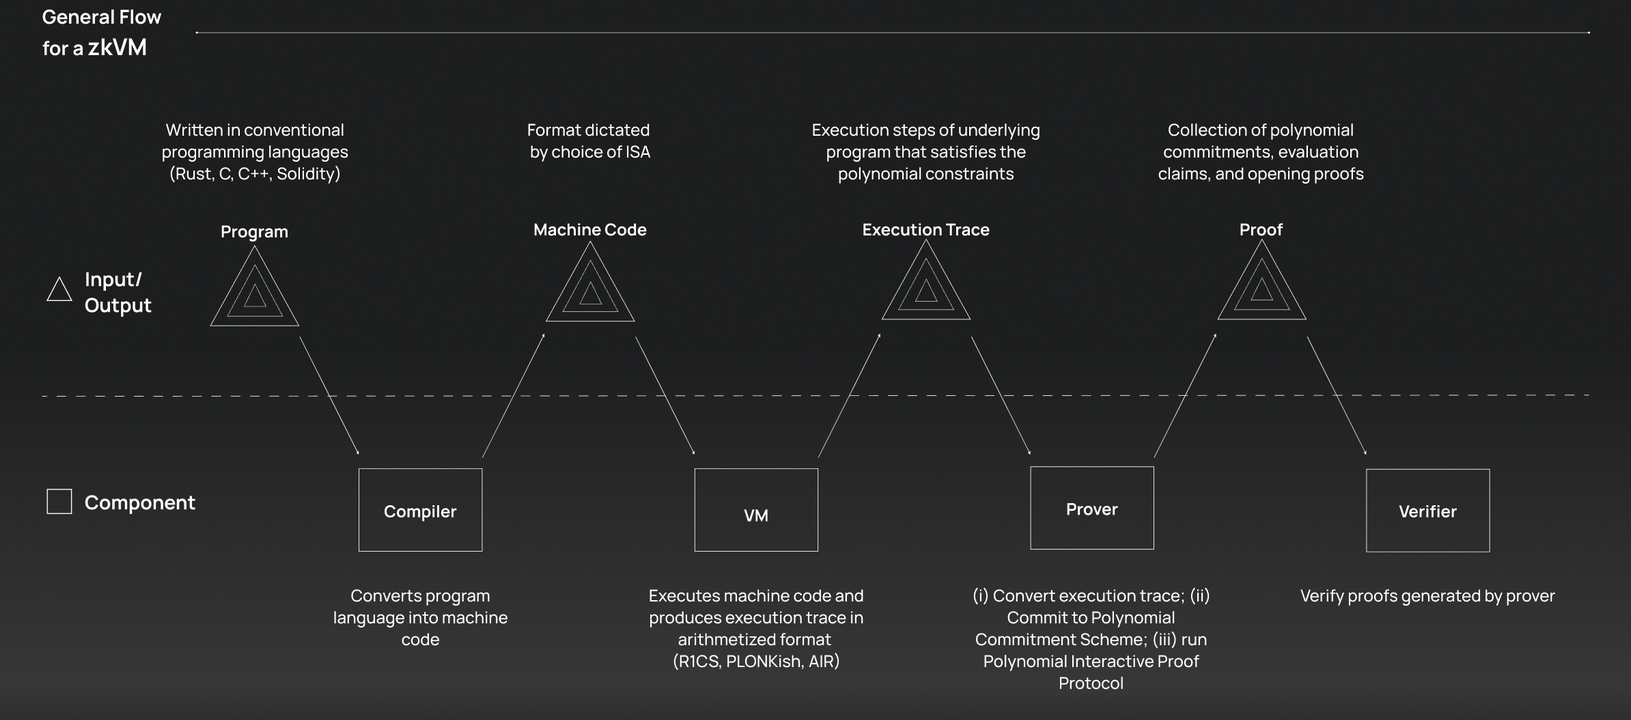
\includegraphics[width=.95\linewidth]{Images/Chap1/zk_worflow.png}
  \caption{Abstract workflow of a zkVM: compilation and local execution (left), trace commitment (centre), and verification (right).\label{fig:zkvm_workflow}}
\end{figure}

The information paths visible in Figure~\ref{fig:zkvm_workflow} can be dissected into four conceptual blocks:
\begin{itemize}
  \item \textbf{Compiler stage:} Source code written in C, C++, Rust, or Solidity is translated into machine code whose exact binary encoding is dictated by the chosen ISA.  Any optimiser run at this level is untrusted; the later stages will still catch mis-compilations because the proof must replay every instruction~\cite{turn0search9}.
  \item \textbf{VM execution stage:}  The zkVM executes the machine code and emits a complete \textit{execution trace}, a row for each clock tick.  The column layout of this table is predetermined by the arithmetisation scheme: R1CS matrices for Groth16, PLONK-ish traces for Halo 2, or AIR tables for plonky2 and RISC Zero \cite{turn0search11}.
  \item \textbf{Prover stage:}
  \begin{enumerate} [label=\textit{(\roman*)}]
      \item The trace is interpolated into a set of polynomials subject to the ISA constraints. 
      \item These polynomials are bound with a polynomial commitment scheme (PCS), yielding a short fingerprint that hides all private rows.
      \item A Polynomial Interactive Oracle Proof (PIOP) is executed in the Fiat–Shamir model, turning the interaction with the verifier into non-interactive challenge hashes. 
      \item Finally, the prover outputs an \textit{opening proof} that convinces any verifier that the blinded evaluations are consistent with the earlier commitment~\cite{turn0search10}.
  \end{enumerate}
  
  \item \textbf{Verifier stage}.  Given the seal, the verifier reconstructs the same challenges, checks the opening proof against the commitment, and either accepts or rejects. Thanks to algebraic batching, only a handful of group or field operations are required, enabling cheap on-chain verification.  
\end{itemize}

A zkVM proof, therefore, certifies that for a \textit{specific} program, and for \textit{some} (undisclosed) input, the recorded execution necessarily produces the claimed public output when run on the stated ISA, without revealing anything else about the private data processed along the way.


\subsection{Historical Evolution of zkVMs}
The trajectory of zero-knowledge virtual machines traces back to the first privacy-preserving roll-ups of 2017–2019, when developers embedded highly specialised circuits, token transfers, Merkle proofs, and mixer arithmetic directly into proving systems.  Such vertical integration proved brittle: every new feature demanded a fresh circuit and weeks of re-auditing. The landscape shifted in 2020 when \textit{Cairo VM} introduced a STARK-friendly, Turing-complete instruction set that powered StarkEx's production roll-ups the very same year, \cite{cairo_starkex,cairo1_blog}. Polygon's announcement of \textit{Miden VM} in 2021 demonstrated that a stack-based ISA, carefully designed for low-degree constraints, could achieve transparent proofs without a trusted setup. In November 2021, the alpha release of Starknet confirmed that general-purpose contracts could run under zero knowledge without bespoke circuits\,\cite{starknet_alpha}.  Early 2022 brought the open-source debut of \textit{RISC Zero}, which executes unmodified 32-bit RISC-V binaries, stitches STARK segments recursively, and finally wraps them with Groth16 to compress the seal to roughly one kilobyte\,\cite{risc0_design_blog} (this is the proof system used for \textit{zkpoex} as explained more in depth in section \ref{proof_system}).  The launch of \textit{zkSync Era} in March 2023 added a byte-accurate zkEVM aimed at mainstream Solidity developers\,\cite{zksync_era}.  Succinct's \textit{SP1} (2024) then layered Nova-style folding on a custom trace format, reaching laptop-grade proving throughput while remaining fully open-source\,\cite{succinct_sp1}.  By 2024, the community gradually distinguished \textit{zkVMs} (language-agnostic, general-purpose) from \textit{zkEVMs} (EVM-specific) to clarify design trade-offs:
\begin{itemize}
    \item \textbf{zkEVMs} prioritize Ethereum compatibility, enabling seamless porting of Solidity contracts but inheriting the EVM's inefficiencies (e.g., stack-based architecture, high opcode complexity)~\cite{zksync_era}. Projects like zkSync and Polygon zkEVM fall into this category, optimizing for developer familiarity~\cite{polygon_miden}.
    
    \item \textbf{zkVMs} (e.g., RISC Zero, SP1) favor flexibility, supporting arbitrary binaries (Rust, C++) and enabling novel use cases like \textit{zkpoex}. They avoid EVM constraints, often achieving better proving efficiency ~\cite{succinct_sp1}.
\end{itemize}

For \textit{zkpoex}, a zkVM was chosen over a zkEVM for three reasons:
\begin{enumerate}
    \item \textbf{Performance}: The Rust-based EVM emulator (\ref{rustevm}) ran more efficiently on RISC Zero's RISC-V ISA than on an EVM-equivalent architecture~\cite{turn0search9}.
    
    \item \textbf{Generality}: \textit{zkpoex} required custom constraints (e.g., reentrancy detection) that were easier to implement in a zkVM's flexible proving environment~\cite{turn0search10,turn0search11}.
    
    \item \textbf{Toolchain Maturity}: RISC Zero's Rust SDK and composable proof system (STARK$\rightarrow$SNARK) simplified integration with existing security tooling \cite{risc0_design_blog}.
\end{enumerate}

This divergence reflects a broader trend: zkEVMs dominate L2 scaling, while zkVMs enable applications beyond Ethereum.

\subsection{Evaluation Criteria for zkVMs}\label{subsec:zkvm_eval}
When comparing zero-knowledge virtual machines, it is tempting to look only at prover speed, yet practical deployments reveal a richer set of trade-offs.  
It's interesting how the Lita Team\footnote{The Lita Team is a team of computer scientists and applied cryptographers dedicated to building the verifiable computer of the future.} defined a holistic approach to evaluating zkVMs. They group the most relevant properties into two families, \textit{baseline reliability} and \textit{performance}, and argue that both must be inspected before declaring one design “better” than another.

\paragraph{Baseline reliability:}
These attributes determine whether a zkVM can be trusted at all.

\begin{itemize}
  \item \textbf{Correctness.}  
        The virtual machine must execute the guest program exactly as specified, and the proof system must uphold its three pillars:  
        \textit{soundness} (false statements cannot be proven),  
        \textit{completeness} (every true statement is in principle provable),  
        and \textit{zero-knowledge} (the proof leaks no information beyond the claimed public output).  
        Failing any pillar turns the system into a liability rather than an asset.
  \item \textbf{Security level.}  
        Each pillar carries a statistical bound.  
        Practice accepts a failure probability of at most \(2^{-n}\) for some security parameter \(n\); higher \(n\) yields stronger guarantees but increases proving effort.  
        Modern STARK-to-SNARK hybrids aim for \(n\ge 96\) bits as a sensible minimum.
  \item \textbf{Trust assumptions.}  
        Proof systems fall into three buckets.  
        Designs with \textit{no trusted setup} rely only on public randomness.  
        Systems with a \textit{one-out-of-(N)} assumption require at least one honest participant in a multi-party ceremony.  
        Block-production schemes may add an \textit{honest majority} assumption.  
        All else equal, fewer assumptions imply a more robust zkVM.
\end{itemize}

\paragraph{Performance metrics:}
Once baseline reliability is satisfied, attention shifts to resource economics.

\begin{itemize}
  \item \textbf{Efficiency.}  
        Core-time per trace row matters for energy-sensitive workloads that must keep proving costs predictable and low.
  \item \textbf{Throughput (speed).}  
        Latency-sensitive applications such as high-frequency trading prefer raw wall-clock speed even at the cost of higher energy consumption.
  \item \textbf{Succinctness.}  
        Proof size and on-chain verification cost dominate user fees for public blockchains.  
        Pairing-based wrappers typically shrink seals to \(\approx1\)\,kB and two pairings, whereas fully transparent STARKs remain in the tens of kilobytes.
\end{itemize}

In practice, the ideal balance depends on the concrete use case.  
Price-sensitive archival systems may favour core-time efficiency, while DeFi protocols gravitate toward minimal latency.  
Developers must therefore benchmark candidate zkVMs across \textit{all six} axes before committing critical workloads.

\begin{figure}[h]
  \centering
  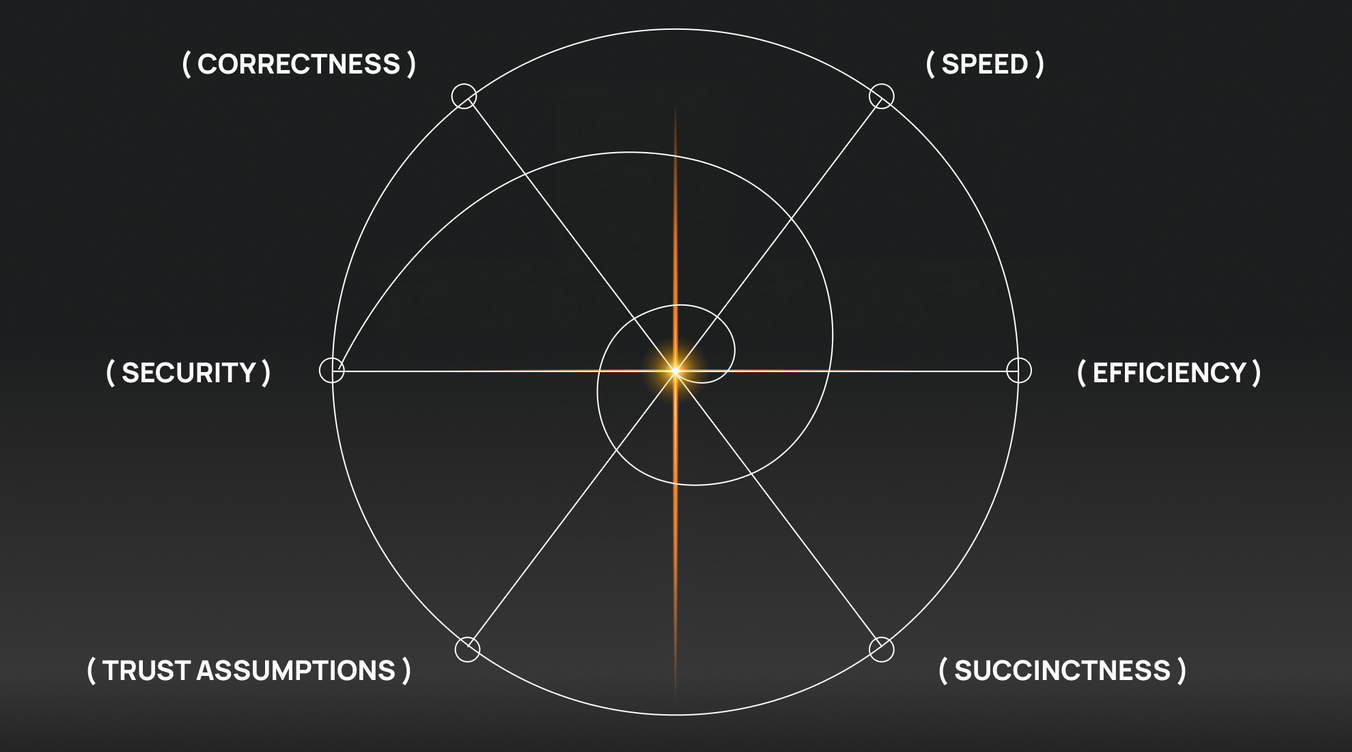
\includegraphics[width=0.8\linewidth]{Images/Chap1/zkVM_axes.png}
  \caption{Radar chart of the six evaluation axes: correctness, speed, efficiency, succinctness, trust assumptions, and security; used to benchmark a zkVM. \cite{lita_zkvm_part1}}
\end{figure}


\subsection{The zkVM Trilemma}
Designers confront three competing objectives:
\begin{enumerate}
  \item \textit{Prover throughput}: hash-based STARK commitments parallelise well on GPUs but emit proofs measuring tens of kilobytes;
  \item \textit{Proof size and verification cost}: pairing-based SNARK wrappers shrink the proof to \(\approx1\)\, kB and verify with two pairings, yet add cryptographic overhead at prove-time;
  \item \textit{Guest compatibility}: byte-accurate zkEVMs reuse existing tooling but inherit an awkward gas-charging microcode, whereas bespoke ISAs simplify constraint systems but require developers to recompile, or even rewrite their contracts.
\end{enumerate}
No implementation hits all three vertices at once: RISC Zero favours small seals and broad language support at the expense of higher prover cycles, while Cairo accepts larger proofs in exchange for maximal throughput.  
The trade-off between these three objectives is well summarized in Figure \ref{fig:zkvm_trilemma}.

\begin{figure}[h]
  \centering
  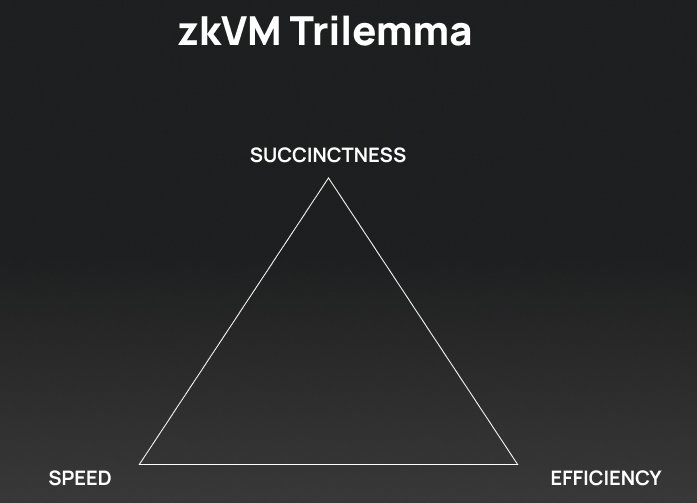
\includegraphics[width=0.7\linewidth]{Images/Chap1/zk_trilemma.png}
  \caption{The zkVM design trilemma: trade-offs between prover speed, proof succinctness, and guest-level compatibility.\label{fig:zkvm_trilemma}}
\end{figure}
